\begin{figure}[t]
\centering
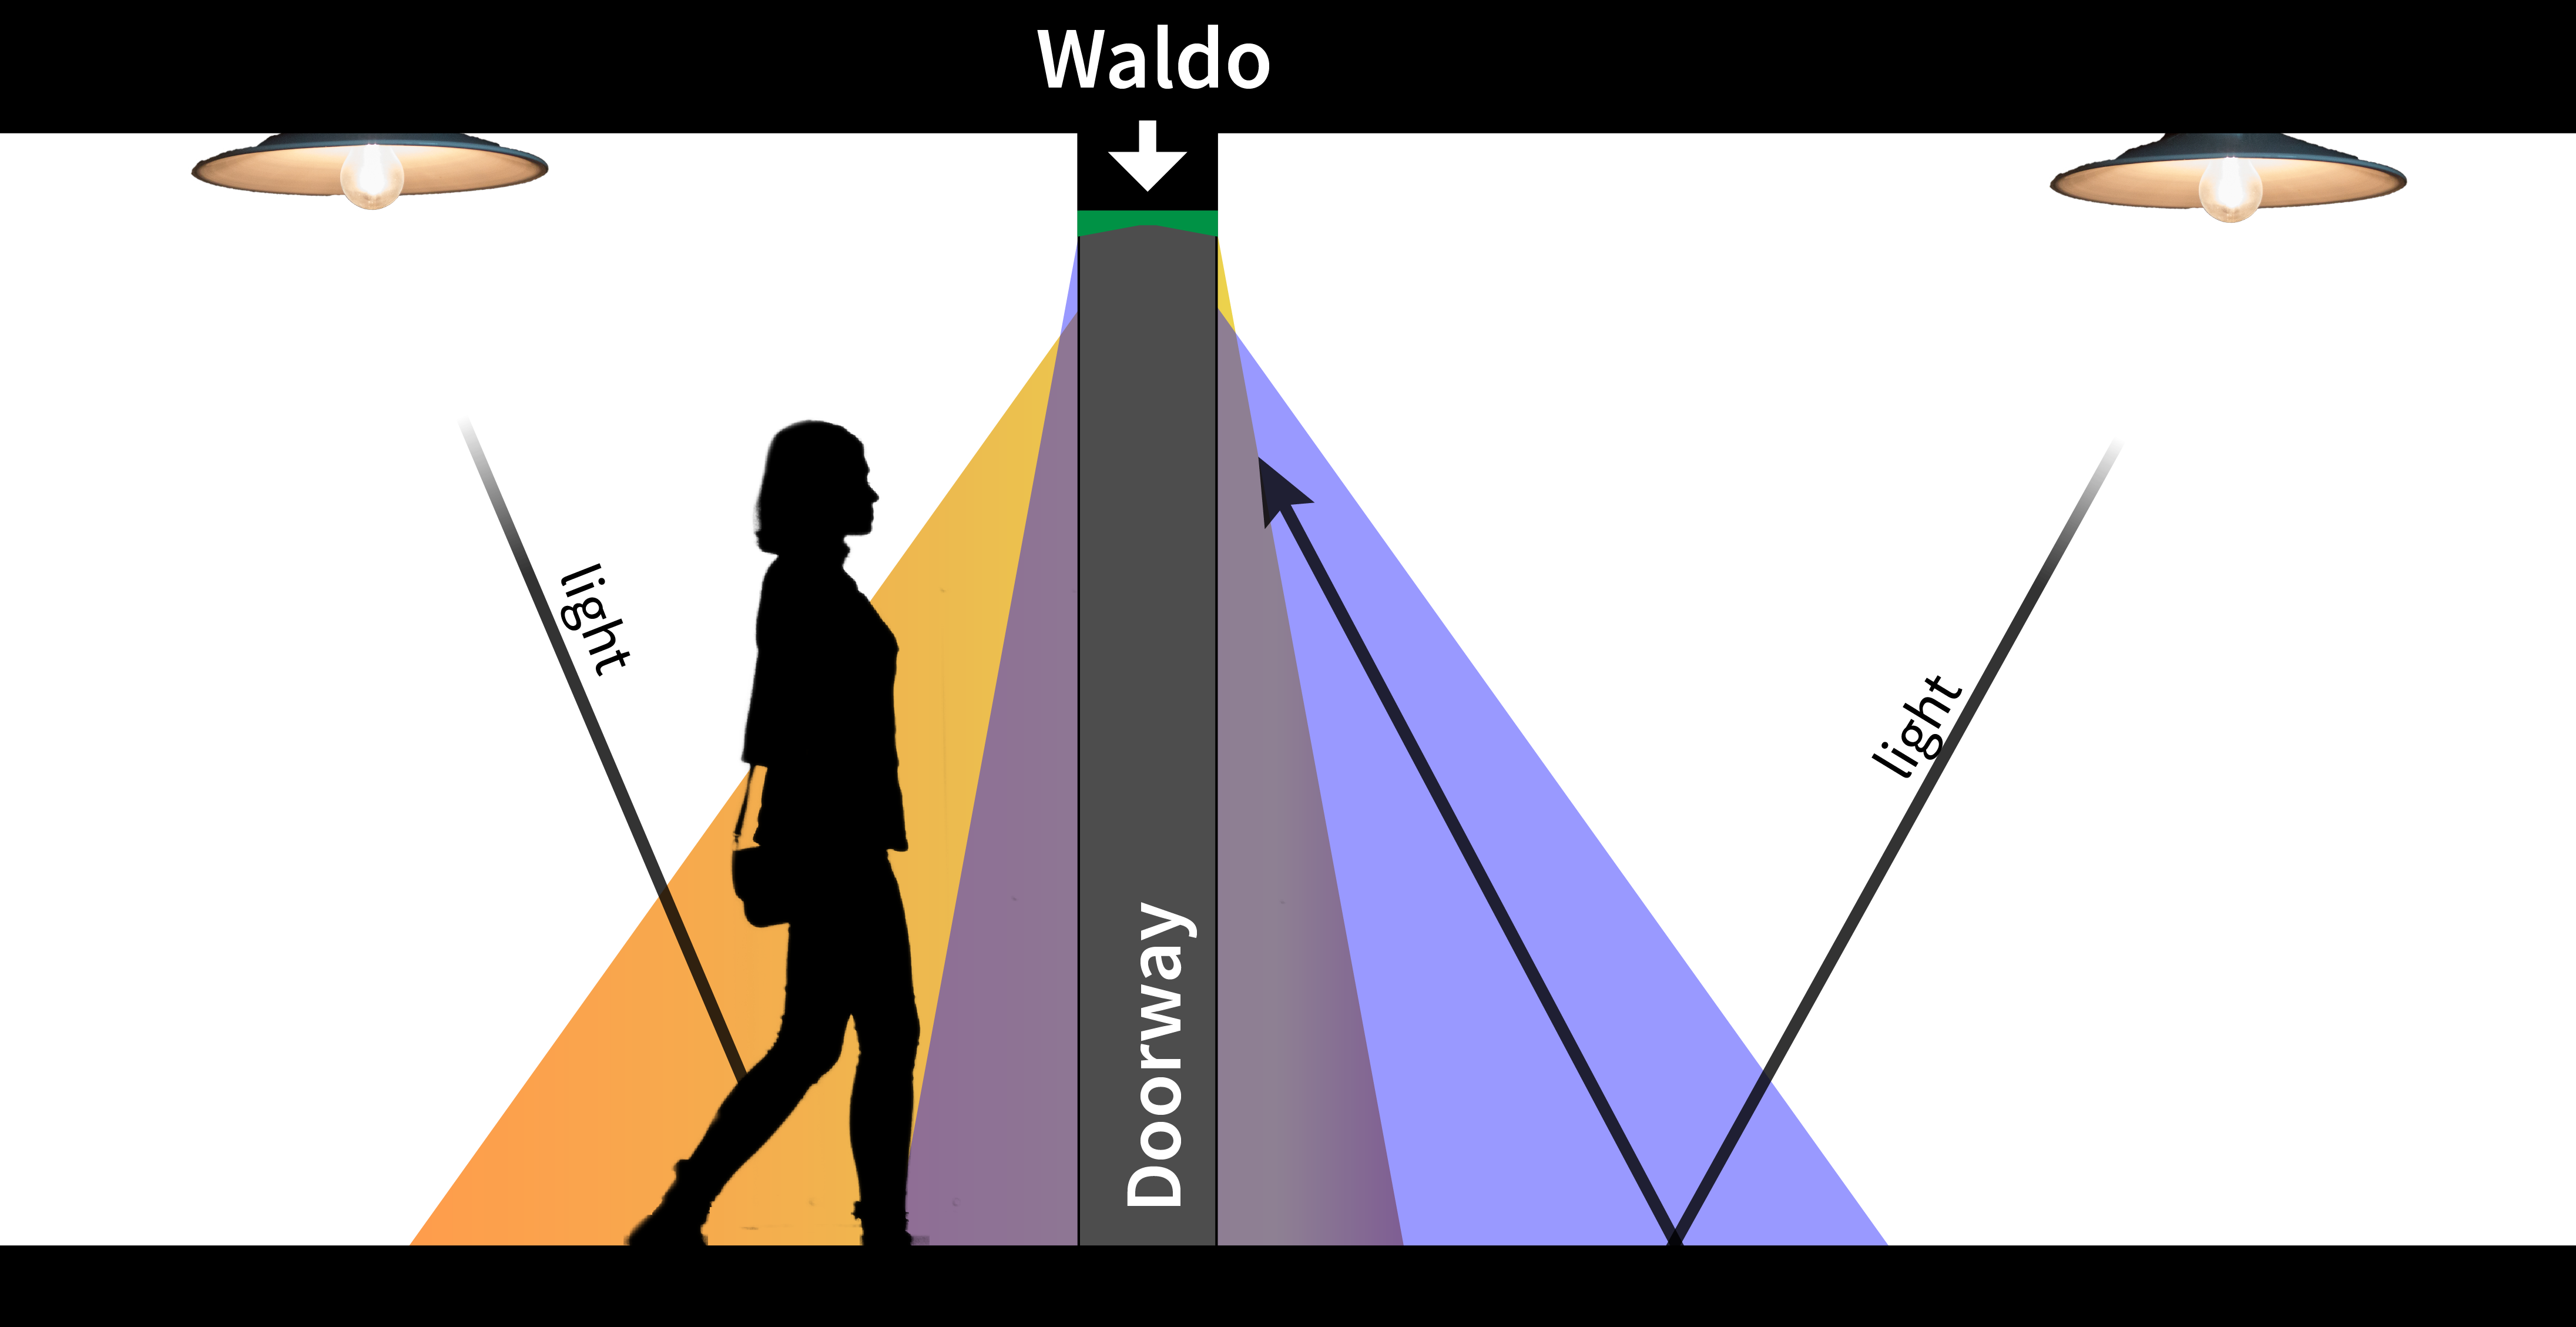
\includegraphics[width=\columnwidth]{figs/scenario.png}
\caption{ The overall system concept of \sysname, a batteryless, energy-harvesting, doorjamb mounted occupancy tracking and person detection enabling system.  This system uses reflective indoor lighting to both power the system and detect person entry and exit activity to a room.\label{fig:syspic}}
\end{figure}

\section{Introduction}
\label{sec:intro}

% intro to occupancy tracking
Understanding how occupants move, work, and live within a workplace or residence is essential for enabling health, efficiency, and security applications in smart buildings.
Appliances, computers, lighting, and heating and cooling systems can adapt their behavior depending on the number of occupants, their needs, and the context of their interactions.
Smart buildings can automatically identify indoor traffic patterns, poorly-used space, and congested walkways, generating data that can be used to further understand how people interact with buildings and the different spaces within them.
These benefits are dependent on the data that sensors collect as they observe people moving through a building and their interactions within the space.

Unfortunately, current occupancy-tracking systems are too large and costly to be considered for large-scale deployment, and are too high-maintenance for long-term monitoring.
There are also privacy concerns for occupancy tracking systems that can identify people's daily habits within a building, possibly without their knowledge.
Existing systems use ultrasound\cite{hnat2012doorjamb}, images\cite{tyndall2016occupancy, teixeira2007lightweight}, wearables\cite{fishkin2005hands}, instrumented objects\cite{buettner2009activity}, structural vibrations\cite{pan2016occupant}, and opportunistic data leaked from existing meters and security systems\cite{yangoccupancy2014}.
%\fxnote{[Can we make the above two sentences more crisp? They're too long and we might miss the point if they're inedible - HD]}
Some of these solutions~(like imaging) gather identifiable information.
Others require building remodeling, force users to change their behavior, or require structural models of the building.
For any of these solutions to work, we must either provide wired power to our sensors (which is usually expensive), or use batteries which increase cost, environmental impact, and fire risk, not to mention required replacement every few years~(even rechargeables).

% our solution
In this paper we present \sysname (overview shown in \figref{fig:syspic}), an occupancy monitoring sensor that is low-cost and low-maintenance, preserves occupant privacy, and can operate for decades\footnote{Actual lifetimes depend on environmental conditions, enclosure quality, and rates of decay for silicon and other circuit materials. The point is that the usual bottleneck (the battery) is not there. Lifetimes of 10--50 years are realistic but not guaranteed.} without wired power or batteries.
%

% why batteryless?
%Importantly, \sysname is batteryless to enable the long term deployment at scales required to instrument entire commercial buildings and residential neighborhoods.
%Batteries are expensive, bulky, environmentally unsustainable, and do not have long lifetimes (even rechargeables).
%By leaving the batteries behind, the device power supply becomes intermittent, complicating execution, data collection, energy management, and timekeeping.
%However, the ability for long term deployments at the scales envisioned for the Internet-of-Things provides enough motivation.

Like the UVa doorjamb sensor~\cite{hnat2012doorjamb}, \sysname is attached to a doorjamb and monitors movement in and out of the doorway.
Unlike previous solutions, \sysname does not use active sensors~(like ultrasonic range finders), but instead senses movement using the same ambient and florescent light reflections that power the sensor.
\sysname harvests solar energy from indoor lights to power all operations, and uses a combination of hardware and software techniques to detect human movement and direction as solar energy availability changes.
%Besides harvesting solar energy, \sysname processes in hardware and software the signal generated by an array of solar panels to detect when people enter or exit a room.
%When enough energy is available, and a person is walking through the doorway, \sysname uses ultrasonic range finders to measure the height of the person for identification.
%\sysname stores this information on device, and opportunistically broadcasts occupancy information to the basestation over a radio.


%Because of the incredibly tight energy constraints and unpredictable energy-harvesting conditions, \sysname uses approximate computing concepts to provide value to the global system no matter the energy conditions.
%\sysname dynamically adapts its duty cycle, task schedule, and data-transmission granularity, depending on the energy available.
%If relatively high amounts of energy are available in the environment, then \sysname will use the ranging sensor to get heights for each person passing through the doorway, and will send each passing event over the air through BLE to the basestation.
%If relatively low amounts of energy are available in the environment, then \sysname will turn off the range finder, and use only the passive, zero-energy-cost solar panels to detect passing events.
%Instead of transmitting on each passing event in this low energy state, \sysname instead sends global statistics opportunistically, detailing the number of events or people that have passed since the last interaction.


\subsection*{Contributions}

The contributions of this paper include:

\begin{compactenum}
	\item A novel system design for unobtrusive, long-term, low-cost, zero-maintenance occupancy tracking.
	\item An in-depth analysis of the design considerations for batteryless, intermittently powered continuous sensing systems that have computation and data with high temporal locality that can be broadly applied to other batteryless sensing applications.
	%\item A novel approximate computing method for adapting the duty cycle of batteryless occupancy  sensors depending on energy available, trading off accuracy for energy.
%\fxnote{[We need to reword this - HD]} %  1) record heights, 2) then record each event and report, 3) only report stats of people going in and out
	%\item An investigation of security and privacy considerations stemming from ubiquitous, low cost occupancy sensors.
	\item An implementation, deployment, and evaluation of \sysname that explores the strengths and limitations of our methods.
\end{compactenum}

\noind
\sysname is, to our knowledge, the first batteryless occupancy monitoring system, and demonstrates the potential and usefulness of long-lived, energy-harvesting, batteryless sensing operation in the built environment.
In this paper we present our design, a working prototype, and evaluation results showing efficacy of the approach.


% These types of condensed table of contents in papers communicate essentially nothing, let's not waste the space - JDH
%\noind
%In the following sections, we give background and related works on occupancy detection and batteryless sensing (\secref{sec:background}), outline the \sysname system design (\secref{sec:system}) and implementation (\secref{sec:implementation}), demonstrate the feasibility and general applicability of \sysname in a variety of situations (\secref{sec:evaluation}), discuss limitations, privacy considerations, and future work (\secref{sec:discussion}), and conclude (\secref{sec:conclusions}).
